\section{Models} \label{sec:models}

%\denes{This is where we can still cut out quite a lot if we want to}
We evaluated four models (logistic regression, random forest, SVMs, MLPs) as implemented in  Scikit-Learn  \cite{pedregosa2011scikit}.

\subsection{Logistic Regression}
The logistic function maps the input feature $\underline{x}_i$ to a probability value $p_i$. Values over $0.5$ correspond to the player winning match $i$.  Training minimizes the \textit{logistic loss} function \cite{hazan2014logistic}:
\begin{equation}
    (p) = -\frac{1}{n} \sum_{i=1}^n p_i \log \left( \frac{y_i + 1}{2} \right) + (1-p_i)\log \left( \frac{1-y_i}{2} \right), 
\end{equation}
where $n$ is number of matches, $p_i$ is the predicted probability of a player winning match $i$, and  $y_i$ is as defined in Eq.~\ref{eq:y}. 
%$$
%\begin{gathered}
%    n = \text{number of matches} \\
%    p_i = \text{predicted probability of a player winning match $i$} \\
%    y_i = \text{outcome of match $i$},
%\end{gathered}
%$$

%where a loss function measures the disparity between observations and their estimated fits .

\subsection{Random Forest}
Random forest classifiers consist of an ensemble of simpler decision trees $\{h(\underline{x},\theta_k),\ k=1,...\}$. %, where %the $\{\theta_k\}$ are independent identically distributed random vectors and 
%each tree casts a unit vote for the most popular class at input $\textit{x}$. 
For the $k$th tree, a random vector $\theta_k$ is generated and fitted to produce a classifier $h(\underline{x}, \theta_k)$ \cite{breiman2001random}. During inference, each tree  casts a vote from input $\underline{x}$; the output is decided by a majority vote. Decision trees tend to be simpler to interpret and quicker to train.

\subsection{Support Vector Machines (SVM)}
SVMs have been used for  \textit{tennis} match predictions.
These models identify the optimal hyperplane in the multi-dimensional feature space that separates data points into the two target classes (win, lose). During training, the marginal distance between this decision boundary and the instances closest to the boundary is maximized. %The existence of a decision boundary can allow for any detection of miss-classification. 
SVMs have a choice of \textit{kernels}, including linear, polynomial, sigmoid or a radial basis function
 \cite{cornman2017machine}.

\subsection{Multilayer Perceptron Neural Networks (MLP)}
An MLP is an artificial neural network consisting of an input layer ($\underline{x}$), an output layer (prediction), and  one or more hidden layers in-between. Neurons in consecutive layers are connected (no connections within layers) \cite{noriega2005multilayer}. Each connection has an associated weight. Training an MLP involves adjustments of these weights using backpropagation to minimize the difference between model output and the desired output.

\begin{figure*}[h]
\centering
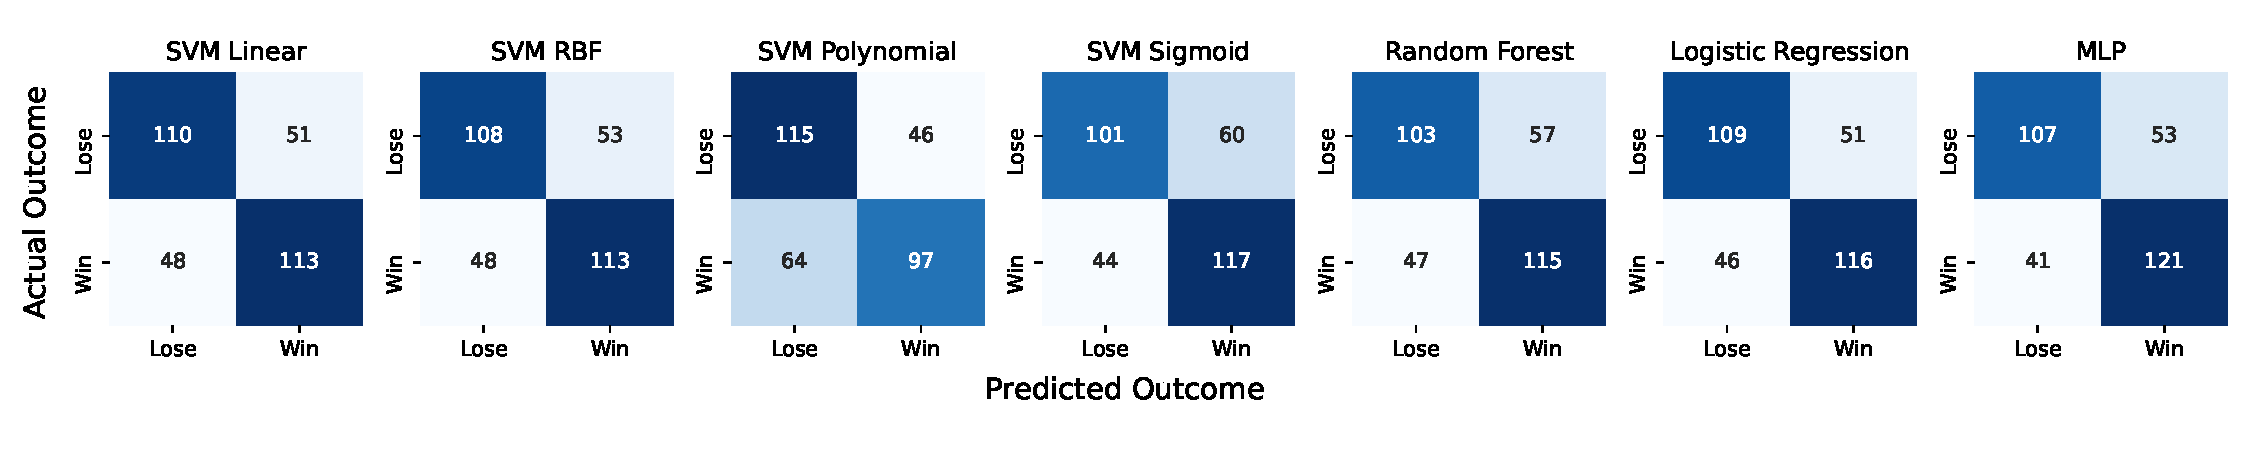
\includegraphics[width=18cm]{plots/chiang6.pdf}
\vspace{-1em}
\caption{Confusion matrices comparing the predicted and actual outcomes of test cases for each trained model.}
%\denes{Please reduce outside margins and consider removing the legend}}

\label{fig:confusionmatrices}
\vspace{-0.2cm}
\centering
\end{figure*}